Qt Creator is our tool of choice for \CPP\ programmming with \US. For non-commercial uses, like ours, Qt Creator is free. Qt Creator is a so-called Integrated Development Environment (IDE). \CPP\-programming requires a variety of tools, varying according to the operating system of both your development environment and of the target system. 

When you download Qt Creator, you will get a version tailored with tools appropriate for your computer (Linux, OS X or Windows). Yet, even for a specific operating system there might be alternative toolsets to choose between. We will be using the toolsets: \concept{MinGW} for Linux and Windows, and \concept{clang} for OS X. If you are an experienced programmer, you may have other preferences which you are welcome to follow.

\section{Install Xcode (Mac OS X only)}
Before you download Qt Creator on OS X, you must install XCode, a free toolset for programming under OS X. To download go to \url{developer.apple.com/download}. Sign in with your Apple ID and follow the instructions to download and install Xcode. The web pages you are lead through are rich with information. See in \iref{fig:xcode} which links and buttons to look for.

\begin{figure} % Side-by-side figures
\centering
\begin{subfigure}{.5\textwidth}
  \centering
  
\includegraphics[width=.9\textwidth]{graphics/xcode-setup-1.png}
  \caption{Step 1.}
\end{subfigure}%
\begin{subfigure}{.5\textwidth}
  \centering
  
\includegraphics[width=.9\textwidth]{graphics/xcode-setup-2.png}
  \caption{Step 2.}
\end{subfigure}
\begin{subfigure}{.5\textwidth}
  \centering
  
\includegraphics[width=.9\textwidth]{graphics/xcode-setup-3.png}
  \caption{Step 3.}
\end{subfigure}%
\begin{subfigure}{.5\textwidth}
  \centering
  
\includegraphics[width=.9\textwidth]{graphics/xcode-setup-4.png}
  \caption{Mission accomplished.}
\end{subfigure}
\caption{Route map to download and install Xcode.}
\label{fig:xcode}
\end{figure}

After installation, launch Xcode. Accept the follow-up instrucions to get Xcode all set. Await the \gui{Welcome to Xcode} (\iref{fig:xcode}) screen, close Xcode, and you are done,

\section{Download Qt creator installer}
You download Qt Creator from \url{www.qt.io/download/}. Navigate to the download page for the open-source version of Qt Creator. It is not always easy to find.

\begin{figure} % Side-by-side figures
\centering
\begin{subfigure}{.5\textwidth}
  \centering
  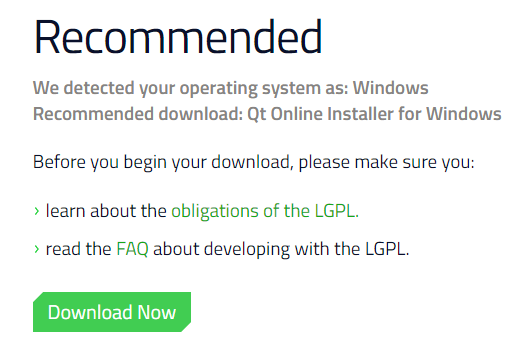
\includegraphics[width=.9\textwidth]{graphics/qt-io-5-win.png}
  \caption{On Windows.}
\end{subfigure}%
\begin{subfigure}{.5\textwidth}
  \centering
  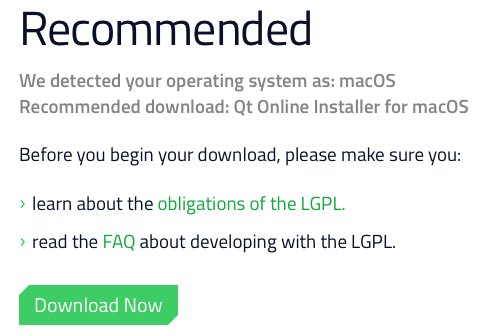
\includegraphics[width=.9\textwidth]{graphics/qt-io-5-osx.png}
  \caption{On OS X.}
\end{subfigure}
\caption{Ready to download Qt Creator.}
\label{fig:qt-recommended}
\end{figure}

The download page will detect your operating system and will arrive at a reasonable suggestion what to download (\iref{fig:qt-recommended}). You finish your task on the web by downloading an installer. Next, run the installer.

%\FloatBarrier
\section{Run Qt Creator installer}

Accept the default suggestions of the installer, except when you come to \gui{Select Components}. Which components to install differ a bit between operating systems. For Windows see \iref{fig:qt-setup-win-1} and \iref{fig:qt-setup-win-2}. For Mac OS X see \iref{fig:qt-setup-osx};

\begin{figure} [h] % Side-by-side figures
\centering
\begin{subfigure}{.5\textwidth}
  \centering
  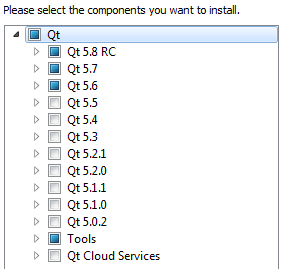
\includegraphics[width=.9\textwidth]{graphics/qt-setup-win-1.png}
  \caption{Default components.}
\end{subfigure}%
\begin{subfigure}{.5\textwidth}
  \centering
  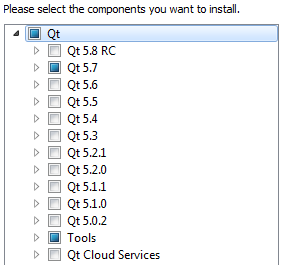
\includegraphics[width=.9\textwidth]{graphics/qt-setup-win-2.png}
  \caption{Unused components have been deselected.}
\end{subfigure}%
\caption{Deselect all other components than \gui{Qt 5.7} and \gui{Tools}.}
\label{fig:qt-setup-win-1}
\end{figure}

\begin{figure} [h] % Side-by-side figures
\centering
\begin{subfigure}{.5\textwidth}
  \centering
  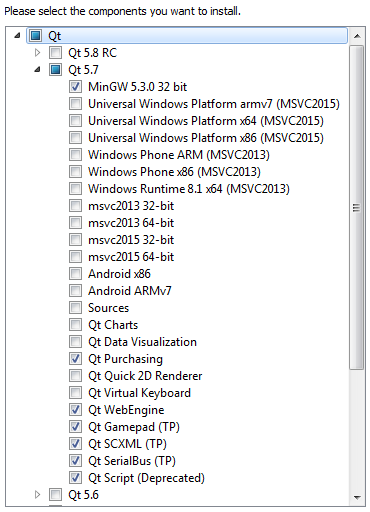
\includegraphics[width=.9\textwidth]{graphics/qt-setup-win-3.png}
  \caption{Default sub-components.}
\end{subfigure}%
\begin{subfigure}{.5\textwidth}
  \centering
  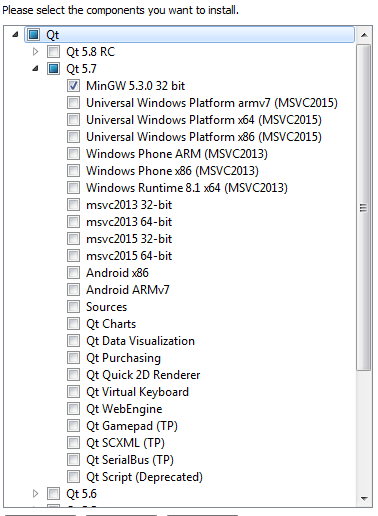
\includegraphics[width=.9\textwidth]{graphics/qt-setup-win-4.png}
  \caption{Unused sub-components have been deselected.}
\end{subfigure}%
\caption{Keep only the \gui{MinGW} sub-component of the \gui{Qt 5.7} component.}
\label{fig:qt-setup-win-2}
\end{figure}

\begin{figure} [h] % Side-by-side figures
\centering
\begin{subfigure}{.333\textwidth}
  \centering
  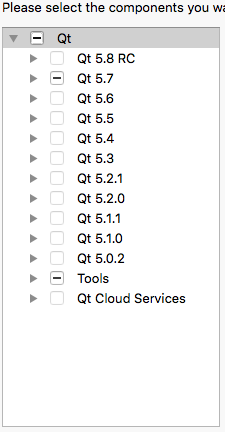
\includegraphics[width=.9\textwidth]{graphics/qt-setup-osx-1.png}
  \caption{Default components.}
\end{subfigure}%
\begin{subfigure}{.333\textwidth}
  \centering
  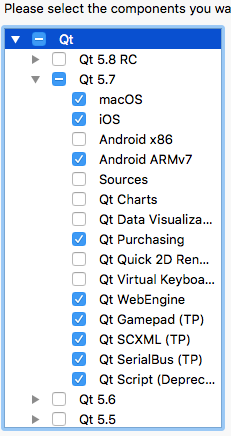
\includegraphics[width=.9\textwidth]{graphics/qt-setup-osx-2.png}
  \caption{Default sub-components.}
\end{subfigure}%
\begin{subfigure}{.333\textwidth}
  \centering
  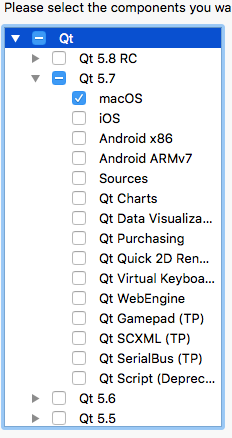
\includegraphics[width=.9\textwidth]{graphics/qt-setup-osx-3.png}
  \caption{Keep only \gui{macOS}.}
\end{subfigure}%
\caption{Keep only the \gui{Qt 5.7} and \gui{Tools} components. Inside \gui{Qt 5.7}, keep only the \gui{macOS} sub-component.}
\label{fig:qt-setup-osx}
\end{figure}

%\FloatBarrier
\section{Final touch}
Accept the final suggestion of the installer to launch Qt Creator. When Qt Creator has launched, right-click its icon in the dock (OS X) or task bar (Windows). On the pop-up menu click \gui{Options} and put a check mark on \gui{Keep in Dock} (OS X). In Windows select \gui{Pin this program to task bar}. 

This procedure will serve to check, that you installed Qt Creator correctly, and will ensure that you can find the program in the dock or task bar, when you need it.

\section{Update system path (Windows only)}
For some reason the installer for Windows does not complete its job. The missing step is to tell Windows where Qt Creator was installed or, more precisely, where the Qt library files were installed. This is accomplished by putting the Qt library folder on the \concept{system path}:

\begin{enumerate}
\item Right-click on \gui{Computer} in File Explorer.
\item Select \gui{Properties}.
\item Select \gui{Advanced System Settings}.
\item Select \gui{Environment Variables}.
\item Under \gui{System variables} select \gui{Path} and then click \gui{Edit...} (\iref{fig:set-system-path-1}).
\item The \gui{Path} variable is specified by a list of folder paths separated by semi-colons. It is a good idea to copy and paste it all to a text editor to get an overview of what's already there (this arcane interface is really a Windows embarressment).
\item The folder likely missing from this list is called \filename{C:/Qt/5.4/mingw491_32/bin} or something similar; the version numbers which will keep incrementing with time. 
\item Find out what the corresponding folder is called on your machine. Use File Explorer to browse inside the \filename{C:/Qt} folder and find it.
\item Return to to \gui{Environment Variables} and add the folder path you just found to the \gui{Path} variable, \eg\ add a semi-colon and then \filename{C:/Qt/5.4/mingw491_32/bin} (\iref{fig:set-system-path-2}).
\end{enumerate}

\begin{figure}
\centering
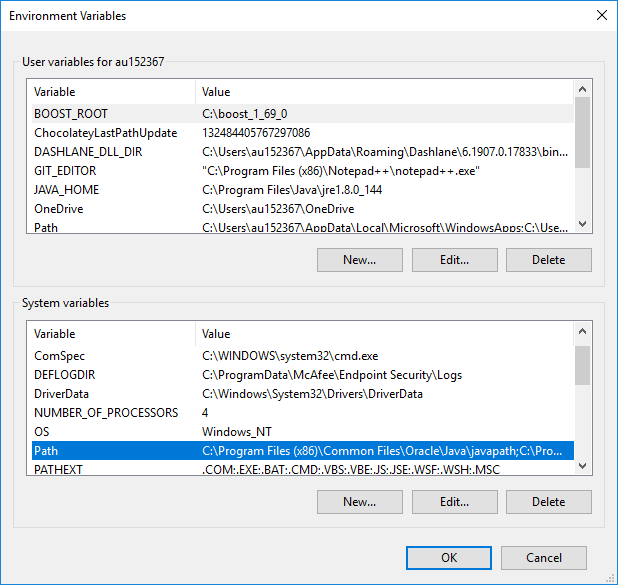
\includegraphics[scale=0.8]{graphics/set-system-path-1}
\caption{Checking the system path on Windows.}
\label{fig:set-system-path-1}
\end{figure}

\begin{figure}
\centering
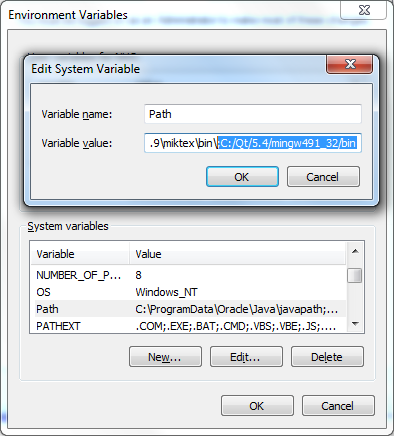
\includegraphics[scale=0.8]{graphics/set-system-path-2}
\caption{Setting the system path on Windows.}
\label{fig:set-system-path-2}
\end{figure}

\section{Upgrading}
You will have reason to re-install and thereby upgrade Qt Creator only rarely. People resort to a re-installation, mostly if Qt Creator should stop working for unknown reasons.

\section{Getting to work}
Before you can begin programming with the \US\ programming framework, remember also to install the Boost library (\iref{ch:install-boost}). Find further instructions in the workflow guidelines (\iref{ch:workflow}).

